\documentclass[a4paper]{standalone}
\usepackage{amsmath}
\usepackage{circuitikz}
\usetikzlibrary{fit, shapes, arrows, patterns, decorations.text, decorations.markings}

\begin{document}
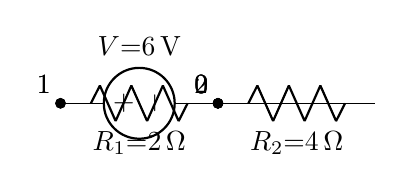
\begin{tikzpicture}[scale=1.00, transform shape, /tikz/circuitikz/bipoles/length=1.50cm, american currents, american voltages, voltage dir=RP]
  \coordinate (1) at (0,0);
  \coordinate (0) at (2,0);
  \coordinate (2) at (2,0);
  \coordinate (0_2) at (4,0);
  \draw[] (0) to [V,l_={$V$}{=$6\,\mbox{V}$},,,,n=V] (1);
  \draw (1) node[circ] {};
  \draw (0) node[circ] {};
  \draw[] (1) to [R,l_={$R_{1}$}{=$2\,\mbox{$\Omega$}$},,,,n=R1] (2);
  \draw (1) node[circ] {};
  \draw (2) node[circ] {};
  \draw[] (2) to [R,l_={$R_{2}$}{=$4\,\mbox{$\Omega$}$},,,,n=R2] (0_2);
  \draw (2) node[circ] {};
  \draw[-, , ] (0) to (0_2);
  \draw (0) node[circ] {};
  \draw[anchor=south east] (1) node {1};
  \draw[anchor=south east] (0) node {0};
  \draw[anchor=south east] (1) node {1};
  \draw[anchor=south east] (2) node {2};
  \draw[anchor=south east] (2) node {2};
  \draw[anchor=south east] (0) node {0};
\end{tikzpicture}
\end{document}